\section{Results}

Following the methodology described in the previous section, we estimate the total U.S. Resource to be 3700 $\pm$400 TWh/yr (Table~\ref{table:totals}). Nearly two-thirds of this is in Alaska where a large resource area and energetic waves in the North Pacific combine to create a large total (2000 - 2550 TWh/yr). The U.S. West Coast has a large remote resource (420 TWh/yr) where energetic waves from the North Pacific arrive from offshore.  The West Coast natural local resource is modest in comparison (90 TWh/yr), but there is potentially another 210 TWh/yr available in the potential resource.

The U.S. East Coast resource, on the other hand, is composed primarily of the local resource (180-230 TWh/yr) and has a relatively modest remote portion (110 TWh/yr). This is because mid-latitude westerly winds tend to generate wave energy that propagates eastward, and relatively less wave energy from the open ocean propagates onshore from the open ocean (i.e., compared to the West Coast). This also indicates that much of the East Coast wave resource is located farther from shore, where there is sufficient fetch to have generated the wave energy. \note{Is that last sentence accurate? Assuming yes, is a citation needed for that or is it `simple physics'-enough to simply be stated?}

Hawaii has a large resource due largely to waves that arrive from the North Pacific along the northern boundary of the EEZ surrounding the islands. The natural local resource is relatively small, due primarily to the fact that the sea-state in this region is -- in the long-average perspective presented here, and compared to regions such as the East Coast where wave growth dominates, or compared to the `potential' case -- roughly `steady-state' because the wind input and dissipation are relatively balanced. The Caribbean region (Gulf of Mexico, Puerto Rico, and U.S. Virgin Islands) on the other hand, has a modest wave resource composed predominantly of local wind input. \note{Is ``the Caribbean region'' a term, or is there something better I should use?} \textcolor{green}{I dont consider GoM to be Caribbean but that might be cultural} The remote resource of this region is also very small because the majority of the U.S. EEZ boundary throughout this region borders other EEZs (rather than being exposed to the open ocean), and the methodology described here only counts wave energy crossing into the EEZ from the open-ocean.

\begin{table}[ht]
  \centering
  \begin{tabular}{|c|c|c|c|c|c|c|}
    \cline{2-7}
    %\multirow{1}{*}{Region}
    \multicolumn{1}{c|}{} & {\it EPRI 2011} & \multicolumn{5}{c|}{New} \\
    \hline
    Region & Remote  & Remote & \multicolumn{2}{c|}{Local} & Total & Inner-Shelf\\
    & & & Natural & Potential & & \\
    \hline
    Alaska & 1570 & 1040 & 990 & 1510 & 2030 - 2550 & 1200 \\
    West Coast & 590 & 420 & 90 & 210 & 510 - 630 & 410 \\
    Hawaii & 130 & 370 & 10 & 100 & 380 - 470 & 120 \\
    East Coast & 240 & 110 & 180 & 230 & 290 - 340 & 90 \\
    Gulf of Mexico & 80 & 13 & 56 & 57 & 69-70 & 20 \\
    P.R. \& U.S.V.I. & 30 & 6 & 11 & 27 & 17 - 33 & 20 \\
    \hline \hline
U.S. TOTAL & 2640 & 1960 & 1340 & 2130 & 3300 - 4090 & 1800 \\
\hline
  \end{tabular}
  \caption{Wave resource assessment results by region and totaled for the entire U.S. (all values in TWh/yr). The range in the total column indicates the sum of Remote+Local (lower value) and Remote+Potential (higher value). \note{Do we need to be more careful w/ significant digits here?}}
  \label{table:totals}
\end{table}

\subsection{Comparing to EPRI 2011}

Our estimate of the total wave energy resource is 25-50\% larger than the EPRI 2011 assessment. This result, however, should not be interpreted too strongly because the majority of this increase is due to including the ``local resource'' over the vast U.S. EEZ, and it is unclear whether this is a technically viable resource. That is, while the energy is theoretically available and contained within U.S. maritime boundaries it is likely to be especially technically challenging to harness.
%In other words, this work has not ``discovered new wave energy'', so much as modified the methodology to account for the wave energy potential over the entirety of the U.S.'s EEZ.

A more realistic near-term assessment of the resource for (i.e., for the next decade or so) is provided in the ``inner shelf'' column, which applies the methodology described in the previous section at 10 nautical-miles from shore, rather than 200. In this case, the remote resource makes up is small for all regions (5\% in Alaska, <2\% for all other regions), so we have only presented the total here. These results are interesting because even though they are composed primarily of the remote resource, several regions (Alaska and Caribbean) actually have a larger inner-shelf than remote resource. This is primarily because the integration contour is longer in these regions than it is at the edge of the EEZ because the contour is not 'clipped' by borders with other nation's EEZs nearly as much as in the full EEZ case.

It is also interesting that the west coast inner-shelf resource (95.5\% remote) is nearly the same magnitude as the resource at the edge of the EEZ. 
\note{GGM: Does this indicate that the resource is fully developed? Or simply  that the way the local resource adds energy doesn't really add much to the resource?}\textcolor{green}{This can be inferred from the difference between natural and potential resource. If both are small then it means that there is little local generation. If potential is much larger than natural then it means the seas were closer to fully developed. That is my interpretation of it, what do you think?} The Hawaiian resource decreases significantly because the 10 nautical-mile boundary is much shorter than the full EEZ boundary (the 10 nautical mile boundary is actually four separate boundaries around island groups). The east coast inner-shelf resource is somewhat smaller than the EEZ remote resource because some of that energy has been removed by whitecapping caused by the westerly winds that create the large local resource in this region (i.e., the westerly winds reduce the energy in westward-propagating waves).

It is also useful to compare the remote results derived here to what was done in EPRI 2011 for two reasons: 1) only the remote resource was computed in that work, and 2) it has been the standard for the U.S. DOE Wave Resource assessment for several years. 
Most regions, except Hawaii, have a lower remote resource compared to EPRI 2011. The reasons for these changes are due to the methodological changes described in section \ref{sec:method:changes}, and all of the changes described there play some role in the final result. However, each region has a {primary \em} reason for the change, and these are discussed in the following paragraph.

The Hawaii resource is the exception to the rule because the EEZ boundary surrounding the State's islands (used here) is much longer than than the 200-m isobath used in the EPRI 2011 results.
Alaska and the West Coast are reduced by approximately 30\%, primarily due to accounting for wave directionality.
The Gulf of Mexico and Caribbean island territories are reduced by large fractions primarily because the integration contour used here is much shorter than was utilized in EPRI 2011. This small integration contour is due to the fact that the majority of the EEZ boundary in these regions is a {\it border} with a neighboring nation's EEZ, and therefore is not considered as described in section \ref{sec:method:calc:remote}.
The East Coast is reduced primarily because this method does not include wave energy that fluxes offshore, which makes up a sizable portion of this region's local resource (i.e., it is counted there, not as part of the remote resource).

Adding the local resource to the total changes the story completely. The magnitude of the local resource for most regions is comparable to the remote resource so that when it is included in the total, it more than makes up for the reduction in the remote resource, which is why the total U.S. resource goes up by 25-50\% compared to EPRI 2011. (alternate wording: total U.S. resource estimate is 25-50\% larger than the EPRI 2011 estimate.)


%\subsection{Wave energy distribution within each region}
\subsection{Natural and potential resource distribution: temporal and spatial}
\note{Levi: I feel like I am just describing the figures, I need to figure out something smart to say. Feel free to chime in}

Bulk power quantities can be used to compare large regions as was done in the previous sections. However the wave resource is not spatially nor seasonally homogeneous. In this section we explore the variability of wave resource in two regions, the West Coast and East Coast. Wave power in the West Coast has a strong seasonal signal with energetic winters and calmer summers (Figure~\ref{fig:maps-wc}). In the Winter, Spring, and Autumn the wave power is stronger offshore Washington and Oregon and weakens southward. These characteristics have been described in previous works \citep[e.g.][]{garcia-medinaWaveResourceAssessment2014,lenee-bluhm_characterizing_2011,yangCharacteristicsVariabilityNearshore2020}. However, during the Summer there is stronger resource offshore California. This is associated with persistent northerly winds that average over 10 m/s during the season (Figure~\ref{fig:maps-wc} second row). The effect of these winds can be seen in areas of increased natural resource that overlap well with the local wind patterns. The potential resource also shows the same pattern during the summer. Similar potential and natural resource indicate that the remote resource is small. On the contrary, offshore Oregon and Washington during the Winter the winds are strong but the natural resource is small. This is because the seas are more developed and local wave growth is not as important. This is further confirmed by a large potential resource in the area. 

% There are two distinct wind patterns in the West Coast. Stronger winds are present in the winter offshore Oregon and Washington and weaken in the summer. Offshore southern Oregon and California the pattern is opposite. Natural resource is largest in the summer than in the winter with the majority of it focused offshore California. The potential resource shows similar behavior to the natural resource but it is stronger in the winter offshore Oregon and Washington. This is because the undisturbed wave field is closer to being in equilibrium, fully developed sea, during this season.

In the East Coast the seasonal cycle of the wind is similar to that of the northern West Coast, with stronger winds in the winter and weaker in the summer (Figure~\ref{fig:maps-at}). The offshore directed winds result in stronger resource near the edge of the EEZ as shown in Figure~\ref{fig:maps-at}. Note that the omnidirectional wave power shows the combined local and remote resource. In general the higher density of natural resource is located offshore of northern New England. In the East Coast, however, the natural resource across the entire area is minimal during the Summer.

% \begin{figure}[ht]
%   \centering
%   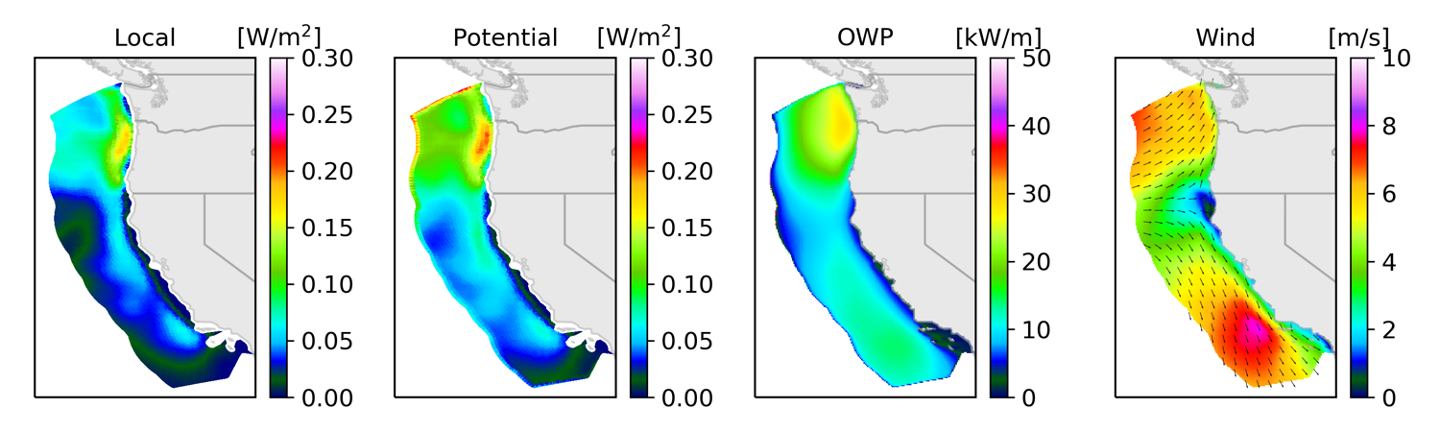
\includegraphics[width=\textwidth]{../fig/WC-Map01-November.png}
%   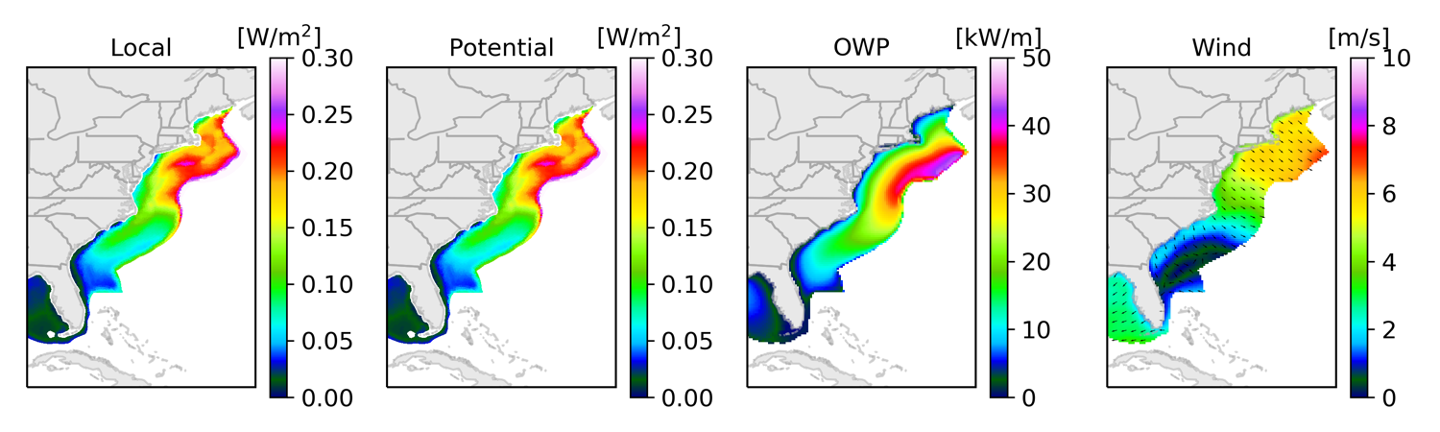
\includegraphics[width=\textwidth]{../fig/EC-Map01-November.png}
%   \caption{Maps of wave resource for the West Coast (top), and East Coast (bottom). \note{GGM: Can we get these as total annual averages, or are those `boring'? Can we add mean wave-direction to the OWP plot?}}
%   \label{fig:maps}
% \end{figure}
% \note{GGM: Regarding Figure \ref{fig:maps}: why are winds and 'potential resource' so different on WC? I would think they would be more spatially correlated? Specifically: why is wind high off of S. Cali, but potential/local resource is highest offshore of OR/WA? ... I think you've answered this question before, but I forget.}

\begin{figure}[ht]
  \centering
  \includegraphics[width=\textwidth]{../fig/wc_spatial_seasonal_mag_4.pdf}
  \caption{Seasonal maps of omnidirectional wave power (top), wind (second row), natural resource (third row), and potential resource (bottom) wave resource for the West Coast. Black contours show areas of 0 $W/m^{2}$ local or potential resource.}
  \label{fig:maps-wc}
\end{figure}

\begin{figure}[ht]
  \centering
  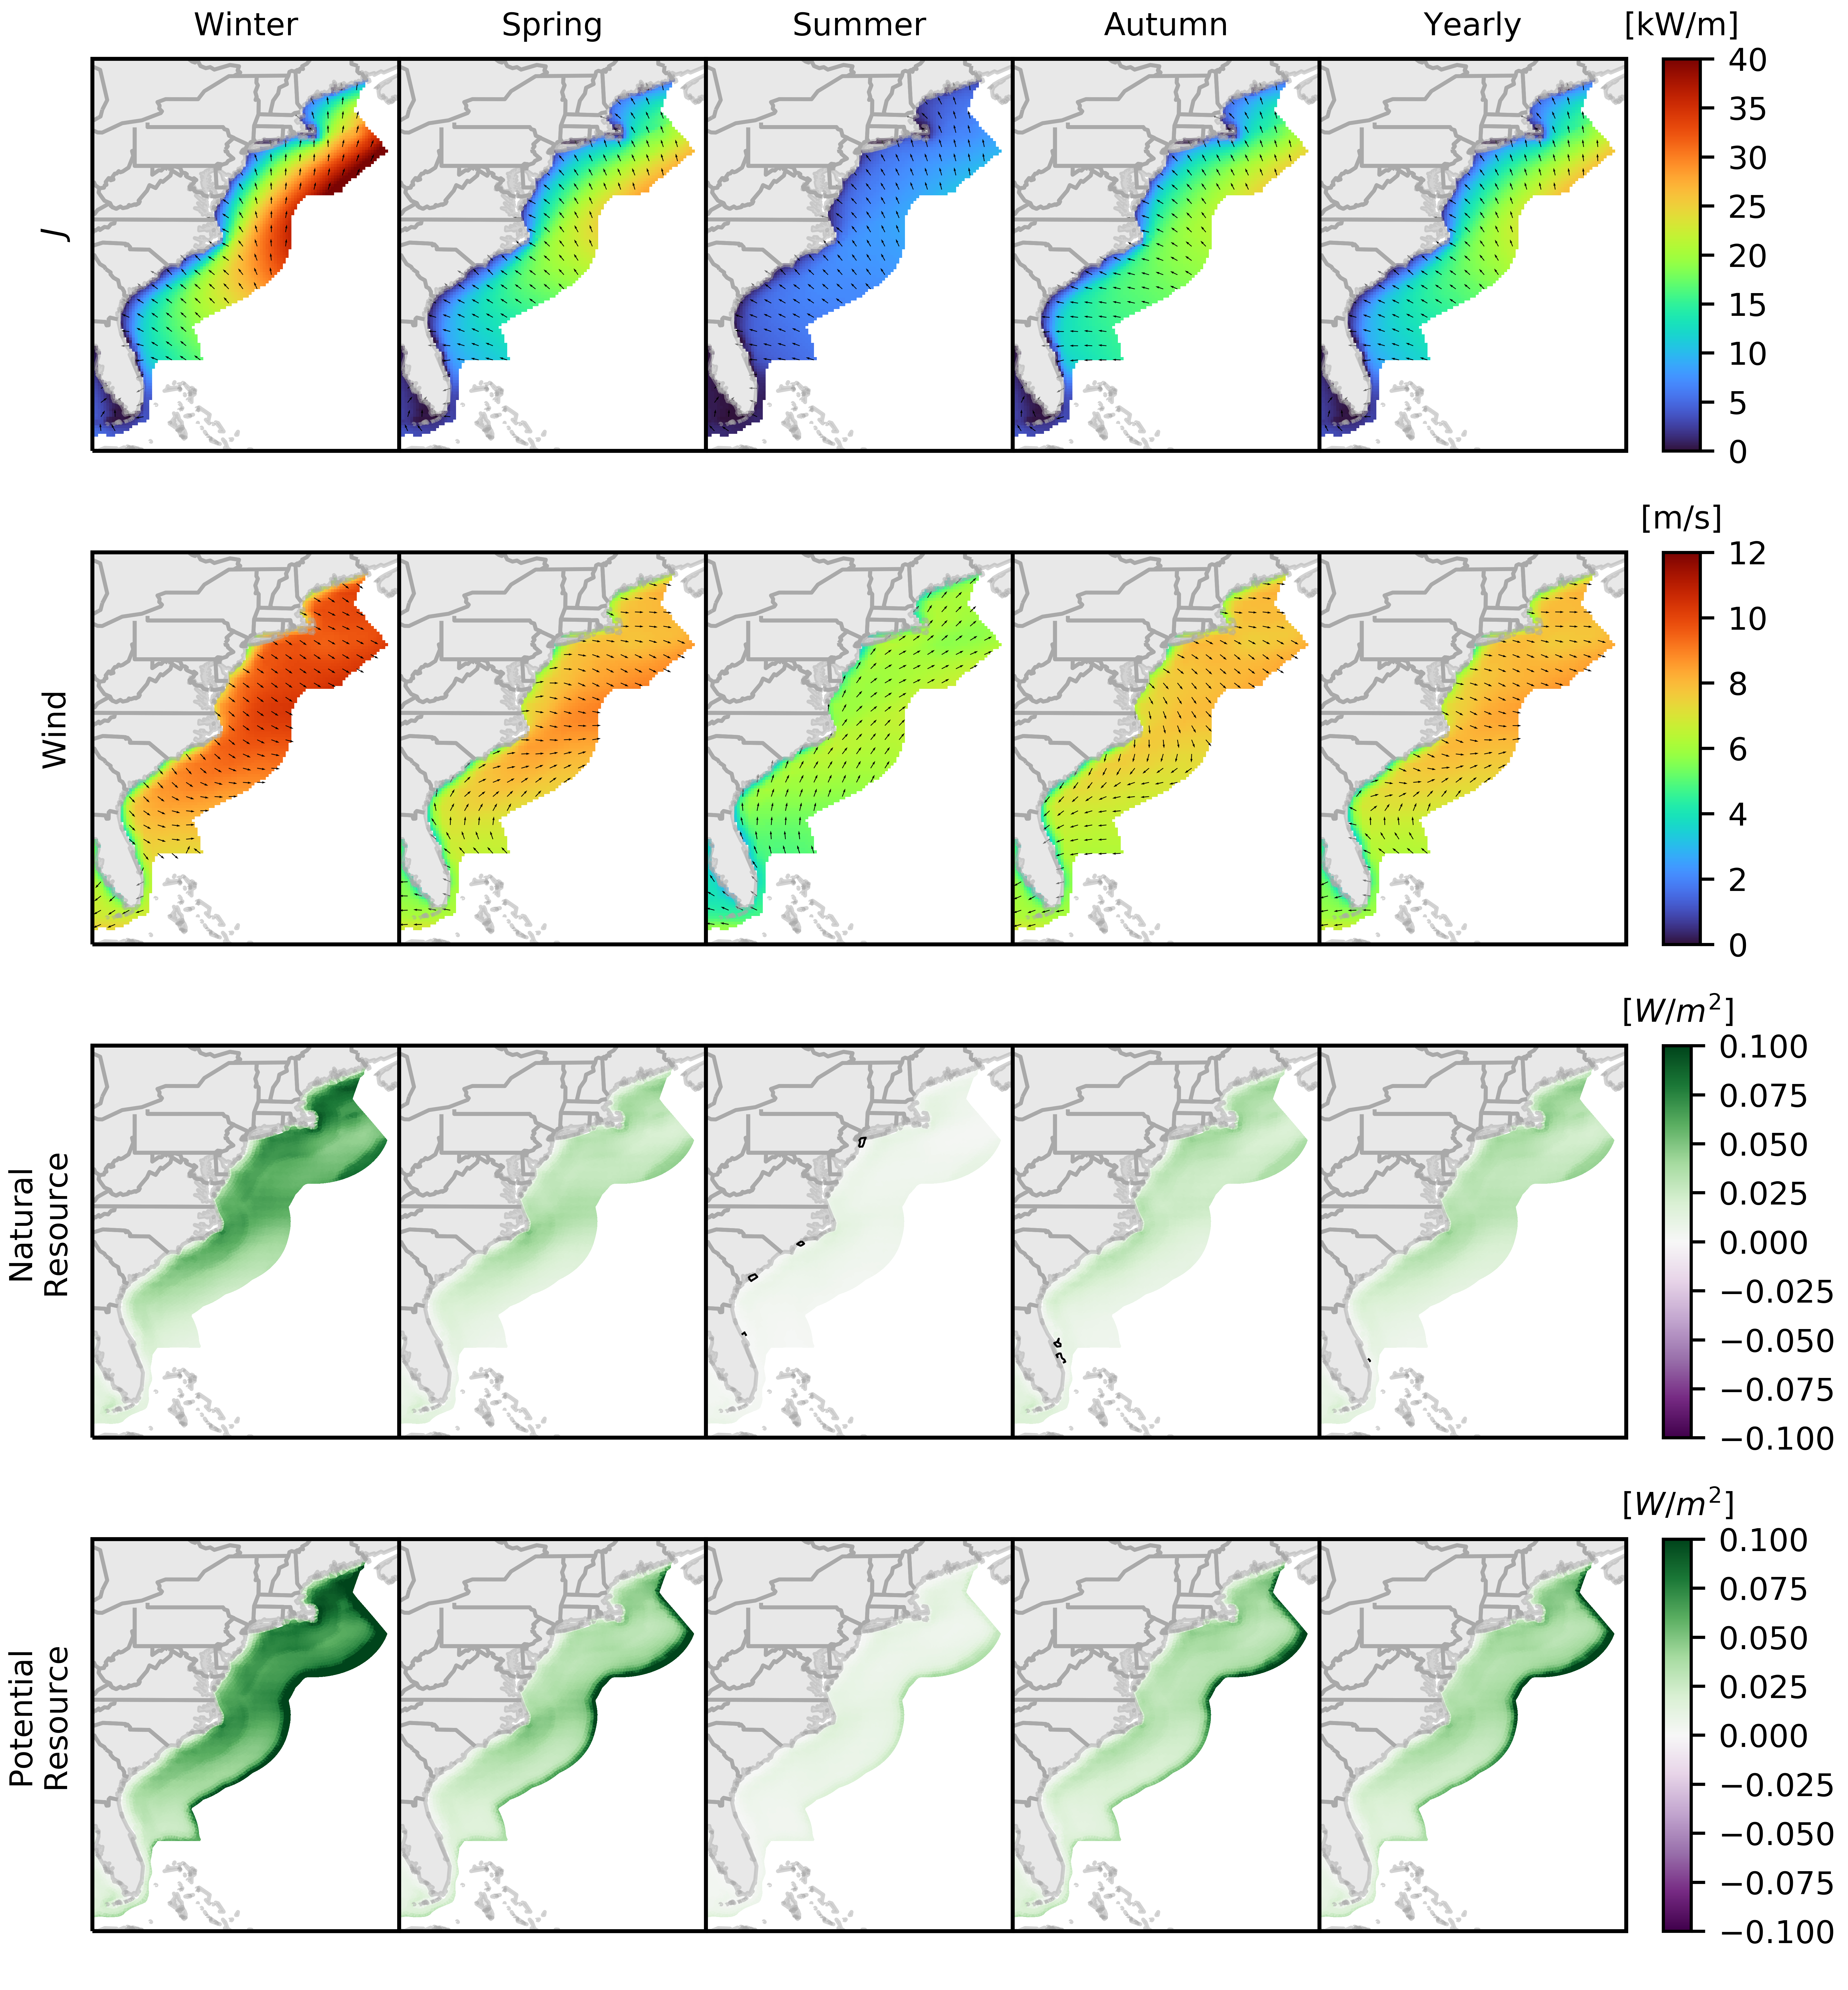
\includegraphics[width=\textwidth]{../fig/at_spatial_seasonal_mag_4.pdf}
  \caption{Same as \ref{fig:maps-at} for East Coast.}
  \label{fig:maps-at}
\end{figure}


Do we want these plots?
\begin{itemize}
\item Plots of ‘remote’ resource vs. distance from shore (Figure 5). ... How does this compare with local resource vs. distance from shore?
\item Remote resource vs. depth. Local resource vs. depth.
\end{itemize}

\subsection{Annual cycle of wave energy resource}

The annual cycle of the wave energy resource has a remarkably consistent pattern across all U.S. regions (Figure \ref{fig:annual-cycle}). Wave energy is a late-fall and winter dominated resource. The resource peaks in December or January across all regions, and is at a minimum in summer months. The inter-annual variability of the monthly-averaged West Coast resource is small during summer months when the resource is small (Figure \ref{fig:wc-variability}). During energetic winter months, the monthly-averaged resource can vary by more than 50\%, but in general the inter-annual variability is less than 30\% of the month's mean. This suggests that during energetic winter months wave energy projects should be expected to deliver at least their annual mean, with the potential of providing up to three-times that value. \note{Is that last sentence a stretch? Am I glossing over too many details about site-specific variability and device performance characteristics?} However, more detailed analysis is required to demonstrate these characteristics at individual sites and for individual technologies. Other regions have similar variability characteristics (not shown for simplicity).

\begin{figure}[ht]
  \centering
  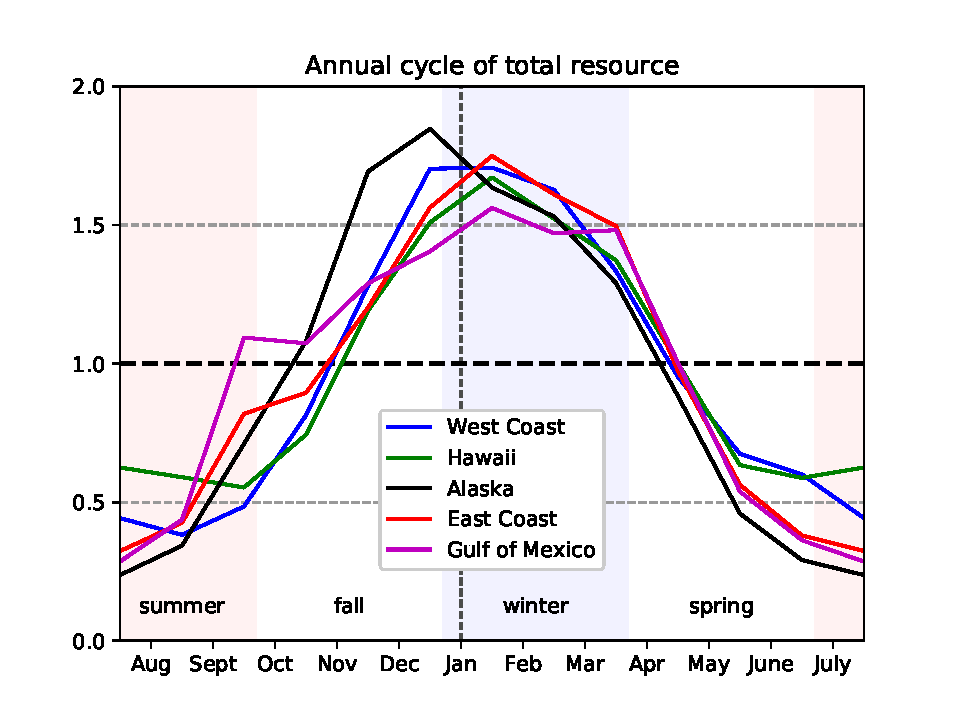
\includegraphics[width=\textwidth]{../fig/AnnualCycle01.pdf}
  \caption[Wave resource annual cycle.]{The annual cycle of the total wave energy resource for several regions, relative to the regional mean.}
  \label{fig:annual-cycle}
\end{figure}


\begin{figure}[ht]
  \centering
  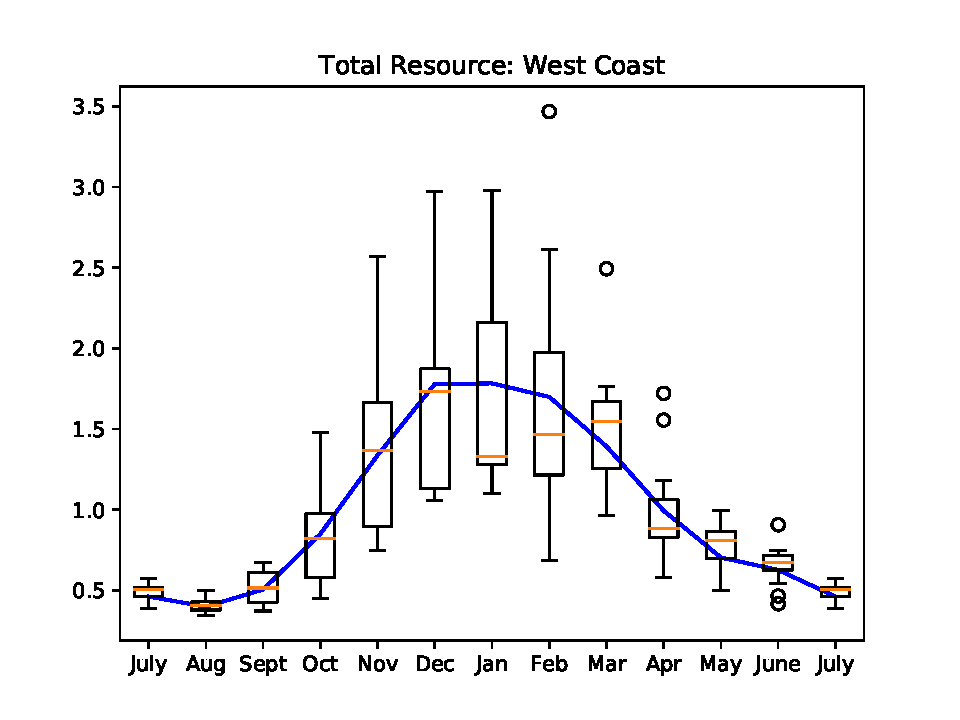
\includegraphics[width=\textwidth]{../fig/AnnualVar01.wc.pdf}
  \caption[West Coast resource variability.]{Annual and inter-annual variability of the West Coast resource. The thick solid line indicates the mean, and the orange lines and boxes indicate the median and quartiles, respectively. The whiskers extend to the last point within 1.5x of the inter-quartile range, and points beyond this are plotted as open-circles.}
  \label{fig:wc-variability}
\end{figure}

\subsection{Wave-period dependence of wave resource}

The US wave energy resource has distinct regional wave-period (frequency) characteristics. The majority of the Gulf (including Puerto Rico and U.S.V.I.) resource is dominated by short-period waves with a peak at ~6.5 seconds, and 95\% of the energy having a period of less than 12 seconds. The West Coast resource has a much wider and longer-period distribution, with 90\% of the resource contained between 6.5 and 19 seconds, with a peak at 14 seconds. This is largely because the west coast resource is dominated by long-period swell that has arrived at the U.S. coastline from storms in the distant Pacific (both North and South Pacific). character.  with 90\% of the resource spanning , on the other hand, lies 

\begin{figure}[ht]
  \centering
  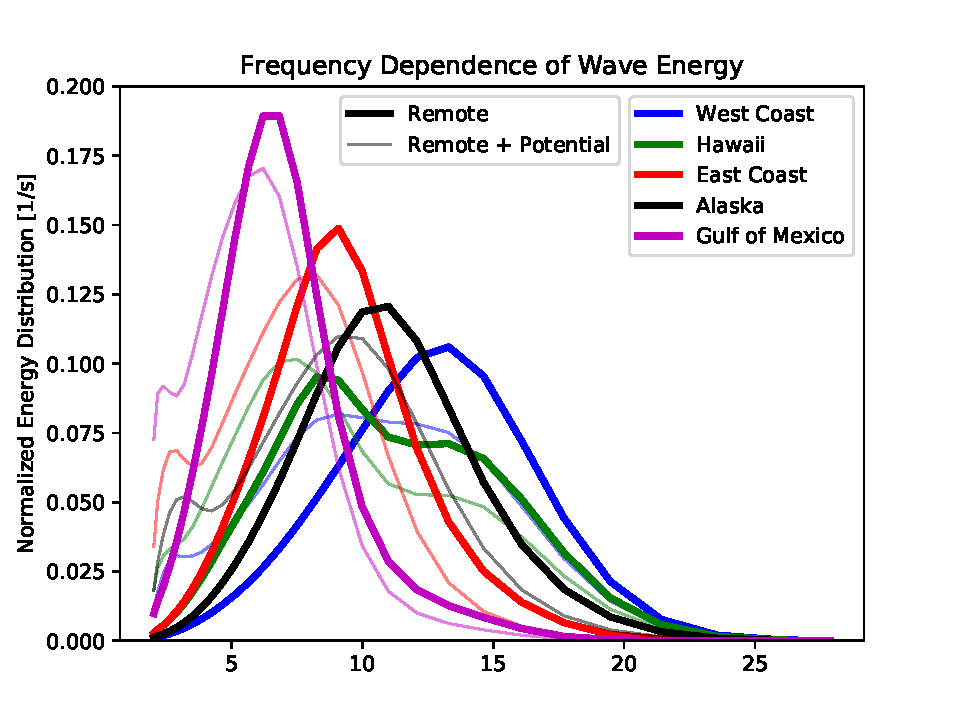
\includegraphics[width=\linewidth]{../fig/TotalResource_Freq02.pdf}
  \caption[Distribution of wave energy vs. wave-period.]{Distribution of wave resource by wave period for each region. Each line represents a spatial average over the entire regional domain. Thick lines indicate the remote resource, thin lines indicate the sum of the potential and remote resource. Colors are used for each region. Each curve is normalized by its total energy (i.e., integral of each curve is 1).}
  \label{fig:remote-freq}
\end{figure}
\note{Does resource look different on N. vs. S. coasts of HI?}


\begin{itemize}
\item Regional differences in frequency dependence?
\item Frequency dependence of local vs. remote?
I don't think we're adding these any more?
\end{itemize}


%%% Local Variables:
%%% TeX-master: "wave_res"
%%% End:
